\documentclass[conference]{IEEEtran}
\IEEEoverridecommandlockouts
\usepackage{cite}
\usepackage{amsmath,amssymb,amsfonts}
\usepackage{graphicx}
\usepackage{textcomp}
\usepackage{xcolor}
\def\BibTeX{{\rm B\kern-.05em{\sc i\kern-.025em b}\kern-.08em
    T\kern-.1667em\lower.7ex\hbox{E}\kern-.125emX}}


\usepackage{caption}
\usepackage{subcaption}
\usepackage{amsthm}

\usepackage[utf8]{inputenc} % allow utf-8 input
\usepackage[T1]{fontenc}    % use 8-bit T1 fonts
\usepackage{hyperref}       % hyperlinks
\usepackage{url}            % simple URL typesetting
\usepackage{booktabs}       % professional-quality tables
\usepackage{amsfonts}       % blackboard math symbols
\usepackage{nicefrac}       % compact symbols for 1/2, etc.
\usepackage{microtype}      % microtypography
\usepackage{xcolor}         % colors

\usepackage{amsmath}
\usepackage{amssymb}
\usepackage{mathtools}
\usepackage{svg}
\usepackage{booktabs}
\usepackage{multirow}

\usepackage{rotating}
\bibliographystyle{IEEEtran}


\renewcommand\thesubfigure{\alph{subfigure}}

\begin{document}

\title{VexDR: $\mathbb V$isually $\mathbb{EX}$plainable $\mathbb D$river Mutation $\mathbb R$ecognition using Whole Slide Images
% \thanks{Identify applicable funding agency here. If none, delete this.}
}

\author{\IEEEauthorblockN{Ho Thi Ngoc Phuong}
\IEEEauthorblockA{\textit{dept. name of organization (of Aff.)} \\
\textit{name of organization (of Aff.)}\\
City, Country \\
email address or ORCID}
\and
\IEEEauthorblockN{Marcel J.T. Reinders}
\IEEEauthorblockA{\textit{dept. name of organization (of Aff.)} \\
\textit{name of organization (of Aff.)}\\
City, Country \\
email address or ORCID}
}

\maketitle

\begin{abstract}

\end{abstract}

\begin{IEEEkeywords}
\end{IEEEkeywords}

\section{Introduction}\label{sec:intro}

Precision oncology depends on identifying tumor-specific molecular alterations (e.g., point mutations, copy-number alterations, and gene fusions) that can be used for diagnosis, prognosis, treatment selection, and trial matching. 
These alterations are not merely associative markers: they are the molecular mechanisms driving tumor growth and progression, making them direct targets for therapy~\cite{sanchez-vegaOncogenicSignalingPathways2018, drilonEfficacyLarotrectinibTRK2018, marabelleEfficacyPembrolizumabPatients2020, mateoDeliveringPrecisionOncology2022}.

In practice, these alterations are diagnosed using molecular pathology assays that range from targeted single-gene tests to broad next-generation sequencing (NGS) panels, whole-exome sequencing, or whole-genome sequencing. 
Although the cost per sequencing run has decreased over time, routine deployment of genome-scale testing still requires substantial investment in bioinformatics infrastructure (compute, storage, pipelines) and specialized personnel to run and maintain these systems.
In their tertiary-hospital implementation study, Kim et al.~\cite{kimClinicalImplementationNextgeneration2025} explicitly highlight both the financial investment required and the bioinformatics specialists and server engineers needed to support NGS in routine care. 
More broadly, the rapid clinical uptake of NGS has created persistent downstream bottlenecks in data processing, quality control, storage, and, most importantly, clinical interpretation of complex variant findings~\cite{karakoyunChallengesClinicalInterpretation2023, remonPrecisionOncologySeparating2018}. 
These deployment barriers (cost and specialized expertise) explain the growing interest in lower-cost triage signals that prioritize which patients warrant confirmatory molecular testing, particularly in settings where universal sequencing is not feasible.

One promising candidate signal is tissue morphology: across several well-studied cancers, driver mutations leave reproducible imprints on H\&E morphology, though the strength, mechanism, and discoverability of these imprints vary by gene, tissue, and cellular context. 
Some associations are mechanistically obligate and pathologist-recognizable 
(CDH1 $\to$ discohesive/lobular~\cite{frixenEcadherinmediatedCellcellAdhesion1991, derksenSomaticInactivationEcadherin2006}; 
VHL $\to$ clear cell~\cite{qiuHIF2aDependentLipidStorage2015, duHIFDrivesLipid2017, chenGYS1InducesGlycogen2020}; 
PML-RARA $\to$ hypergranular promyelocytes~\cite{grignaniFusionProteinsRetinoic1998, linRoleHistoneDeacetylase1998, swerdlowWHOClassificationTumours, sehgalAuerRodsFaggot2023}; 
MYC $\to$ starry-sky Burkitt~\cite{evanInductionApoptosisFibroblasts1992, eischenDisruptionARFMdm21999}). 
For most other recurrent driver mutations (KRAS, EGFR, PIK3CA, TP53, ATM, etc.), the morphological correlates are more subtle and confounded by the cell-of-origin and the subtype context in which the mutation occurs.
These genotype-to-morphology relationships open a complementary triage axis: 
routine H\&E morphology can act as a low-cost triage layer that prioritizes which patients warrant confirmatory molecular testing, provided the imprints, including the subtle and confounded ones, can be extracted reliably and explained in pathologist-interpretable terms.

The last decade has seen a rapid expansion of digital pathology, driven by improvements in whole-slide imaging (WSI) scanners, storage/compute infrastructure, and clinical validation efforts~\cite{vanderlaakDeepLearningHistopathology2021, evansUSFoodDrug2018, mukhopadhyayWholeSlideImaging2018}.
These developments have made computational pathology a natural domain for deep neural networks (DNNs), because DNNs can learn predictive features directly from pixel data at multiple spatial scales~\cite{dimitriouDeepLearningWhole2019}. 
Early work established strong proof-of-concept that clinically relevant molecular alterations are, to some extent, predictable from routine hematoxylin-and-eosin (H\&E) morphology using convolutional neural networks (CNNs) trained on tiled WSIs. 
Coudray et al.~\cite{coudrayClassificationMutationPrediction2018} train a CNN on The Cancer Genome Atlas (TCGA) WSIs and reported that multiple recurrent lung adenocarcinoma gene mutations (including EGFR, KRAS, STK11, and TP53) could be predicted from H\&E with meaningful discrimination performance.
Kather et al.~\cite{katherPancancerImagebasedDetection2020} extend this approach to 14 cancer types in over 5,000 patients, with mean cross-validated AUROCs for the top driver mutations clustering in the 0.6--0.8 range across lung, colorectal, breast, and gastric cancers.
Fu et al.~\cite{fuPancancerComputationalHistopathology2020} show that whole-genome doubling has a universal morphological signature across cancer types. 

Translation to routine clinical workflows, however, has been limited, both because external-cohort generalization remains uneven~\cite{niehuesGeneralizableBiomarkerPrediction2023, arslanSystematicPancancerStudy2024} and because established biomarkers are already covered by mature IHC and ISH assays. 
A separate concern, central to the present work, is that these models offer little mechanistic insight into the genotype-morphology relationships they exploit.
Subsequent work using multiple instance learning (MIL) and attention-based aggregation~\cite{ilseAttentionbasedDeepMultiple2018, luDataefficientWeaklySupervised2021, campanellaClinicalgradeComputationalPathology2019} improve discrimination performance and produced post-hoc attention maps that purport to localize the morphological evidence behind each prediction, although the fidelity of these maps to underlying biology is contested.

A recurring observation across theses efforts is that molecular subtypes are substantially more predictable from H\&E than the individual driver mutations they contain.
Strong subtype-from-H\&E results have now been reproduced for breast intrinsic subtypes~\cite{coutureImageAnalysisDeep2018, naikDeepLearningenabledBreast2020}, colorectal consensus molecular subtypes (CMS)~\cite{bilalDevelopmentValidationWeakly2021, wagnerTransformerbasedBiomarkerPrediction2023}, endometrial ProMisE classes~\cite{volinsky-fremondPredictionRecurrenceRisk2024}, and bladder muscle-invasive subtypes~\cite{woerlDeepLearningPredicts2020}.
Kather et al.~\cite{katherPancancerImagebasedDetection2020} make the same point in their own data, finding that integrated features such as MSI, homologous recombination deficiency, and expression-based subtypes were markedly more predictable than the individual mutations comprising them.
This asymmetry has a straightforward interpretation: each subtype integrates many co-occurring molecular features that push morphology in correlated directions, producing a stronger and more reproducible histologic signal than any single driver. 
A methodological consequence is that some apparent single-mutation predictions are partly subtype prediction in disguise: a model nominally calling TP53 or PIK3CA in breast cancer recovers, in part, the basal-like or luminal-A context in which those mutations are enriched.

A second, more recent shift is the rise of pathology foundation models: 
large self-supervised vision encoders pre-trained on millions of whole-slide 
images across institutions and tissues. 
UNI~\cite{chenGeneralpurposeFoundationModel2024} (100M tiles, 100K slides, 20 tissue types), Prov-GigaPath~\cite{xuWholeslideFoundationModel2024} (1.3B tiles from 171K real-world non-TCGA slides), Virchow~\cite{vorontsovVirchowMillionSlideDigital2024} (a 632M-parameter ViT trained on 1.5M Memorial Sloan Kettering slides), and the open-weights Phikon~\cite{filiotScalingSelfSupervisedLearning2024} have collectively reset the floor for what counts as a strong off-the-shelf representation in computational pathology. 
The vision-language variant CONCH~\cite{luVisuallanguageFoundationModel2024} reports zero-shot subtype classification accuracies above 90\% on NSCLC, RCC, and breast cancer. 
These models substantially mitigate the representation-learning and external-cohort generalization problems that limited the previous CNN/MIL generation. 
They do not, however, resolve the explainability problem: hierarchical attention, joint vision-language pre-training, and patch-level pooling all complicate post-hoc attribution to specific morphological structures, and large-scale pre-training does not by itself guarantee that the features driving a prediction correspond to the biology a pathologist would recognize.


% TODO: contributions (not now, need to wait for the results)

\section{Related Work}\label{sec:related}

\subsection{Genotype, subtype, and morphology}\label{sec:related/morphology}

The literature supports a hierarchical view of the genotype-morphology relationship, from near-obligate, mechanistically-traceable lesions at the top to point mutations with no recognizable imprint at the bottom.

At the top, a small set of genes produce near-pathognomonic morphology in their tissue context.
CDH1 loss disrupts adherens junctions, producing single-cell discohesion characteristic of invasive lobular carcinoma~\cite{frixenEcadherinmediatedCellcellAdhesion1991, derksenSomaticInactivationEcadherin2006}.
VHL loss stabilizes HIF, which induces PLIN2 to package lipid droplets~\cite{qiuHIF2aDependentLipidStorage2015} and represses CPT1A to block fatty acid oxidation~\cite{duHIFDrivesLipid2017}; together with HIF-driven glycogen accumulation~\cite{chenGYS1InducesGlycogen2020, pescadorHypoxiaPromotesGlycogen2010}, this produces the clear cytoplasm of clear cell renal cell carcinoma.
PML-RAR$\alpha$ arrests myeloid maturation at the promyelocyte stage through enhanced corepressor/HDAC recruitment~\cite{grignaniFusionProteinsRetinoic1998, linRoleHistoneDeacetylase1998}, producing the hypergranular promyelocytes with faggot cells characteristic of acute promyelocytic leukemia~\cite{swerdlowWHOClassificationTumours, sehgalAuerRodsFaggot2023}.
MYC deregulation couples proliferation with apoptosis~\cite{evanInductionApoptosisFibroblasts1992, eischenDisruptionARFMdm21999}; combined with cooperating mutations, it produces Burkitt lymphoma~\cite{schmitzBurkittLymphomaPathogenesis2012}, where high cell turnover generates the characteristic starry-sky pattern of tingible-body macrophages clearing apoptotic cells~\cite{swerdlowWHOClassificationTumours, dy-ledesmaStarrySkyPattern2016}.
The lesion–morphology association recurs across many tumor types:
the DNAJB1-PRKACA fusion is present in essentially all fibrolamellar hepatocellular carcinomas~\cite{honeymanDetectionRecurrentDNAJB1PRKACA2014}, which are defined by their lamellar-fibrosis architecture~\cite{craigFibrolamellarCarcinomaLiver1980}; 
germline FH mutation followed by somatic loss of the second allele~\cite{tomlinsonGermlineMutationsFH2002} drives fumarate accumulation~\cite{pollardAccumulationKrebsCycle2005, adamRenalCystFormation2011} and is associated with the inclusion-like nucleolar morphology recognized as the hallmark of HLRCC RCC~\cite{merinoMorphologicSpectrumKidney2007}; 
the ETV6-NTRK3 fusion produces the microcystic, secretion-rich morphology shared by secretory breast carcinoma~\cite{tognonExpressionETV6NTRK3Gene2002} and its salivary-gland counterpart, mammary analogue secretory carcinoma (MASC)~\cite{skalovaMammaryAnalogueSecretory2010}.
In each case a single defining lesion, which either disrupts a tissue-specific differentiation program or imposes an obligatory metabolic or architectural phenotype, is associated with morphology that a pathologist can recognize at low magnification.

Beneath this layer, the link weakens from obligate to probabilistic: a subtype enriches for a recognizable morphologic cluster, but the same morphology can arise outside it and a member of that subtype can present without it. 
In breast cancer, the PAM50 intrinsic subtypes~\cite{parkerSupervisedRiskPredictor2009} partition tumors along an axis of luminal differentiation: luminal tumors retain ESR1, GATA3, and FOXA1 expression, while basal-like tumors lose this program and present as high-grade carcinomas~\cite{koboldtComprehensiveMolecularPortraits2012} with medullary-like features~\cite{livasyPhenotypicEvaluationBasallike2006}.
Deep learning can partially recover this signal from H\&E at $\approx$77\% accuracy for the binary basal-vs-non-basal call~\cite{coutureImageAnalysisDeep2018} and $\approx$66\% for the four-class call~\cite{jaberDeepLearningImagebased2020}.
In colorectal cancer, the four consensus molecular subtypes, including MSI immune (CMS1), WNT/MYC canonical (CMS2), KRAS metabolic (CMS3), and TGF-$\beta$ mesenchymal (CMS4)~\cite{guinneyConsensusMolecularSubtypes2015}, leave H\&E imprints (Crohn-like lymphoid infiltrates in CMS1~\cite{greensonPathologicPredictorsMicrosatellite2009}; desmoplastic stroma in CMS4~\cite{isellaStromalContributionColorectal2015}) that the imCMS classifier~\cite{sirinukunwattanaImagebasedConsensusMolecular2021} predicts at macro-AUROC $\approx$0.84 on held-out cohorts.
In endometrial cancer, the four TCGA molecular classes cluster along axes of mutational load and chromosomal stability: POLE-ultramutated and MMRd hypermutated tumors carry high neoantigen loads and dense TILs~\cite{howittAssociationPolymeraseEMutated2015}, while p53-abnormal copy-number-high tumors display marked nuclear atypia and serous-like architecture~\cite{levineIntegratedGenomicCharacterization2013, fremondInterpretableDeepLearning2023}. Pathologist discordance motivated the molecular reclassification~\cite{gilksPoorInterobserverReproducibility2013}; all four classes can now be predicted from H\&E~\cite{fremondInterpretableDeepLearning2023} as a component of the HECTOR recurrence prognosticator~\cite{volinsky-fremondPredictionRecurrenceRisk2024}.
The pattern recurs in thyroid cancer, where BRAF V600E drives strong MAPK activation and the classical-type papillary architecture while RAS-family mutations produce weaker MAPK signaling and a follicular-pattern morphology~\cite{agrawalIntegratedGenomicCharacterization2014}, and in small cell lung cancer, where the ASCL1-, NEUROD1-, POU2F3-, and YAP1-defined transcriptional subtypes are defined transcriptionally rather than morphologically~\cite{rudinMolecularSubtypesSmall2019}.
In each case the morphology emerges from the aggregate of co-occurring alterations and the transcriptional program they engage; no single mutation suffices to produce it.
This is why subtype prediction from H\&E achieves consistently higher within-cohort AUROCs than individual-mutation prediction, even when the same model architecture is used for both targets~\cite{katherPancancerImagebasedDetection2020, arslanSystematicPancancerStudy2024}.

At the bottom of the hierarchy, most somatic point mutations have no human-recognizable morphologic signature and are predictable from H\&E only via cell-of-origin, subtype enrichment, or coincidental association with a more morphologically penetrant alteration.
Pan-cancer integrative analyses confirm that cell-of-origin, not individual driver mutations, dominates the molecular taxonomy of human tumors~\cite{hoadleyCellofOriginPatternsDominate2018}, and the same asymmetry is observed when the predictor is H\&E: pan-cancer studies that train one model per recurrent driver mutation report AUROCs clustered in the 0.6--0.8 range, with mean single-nucleotide-variant performance materially lower than subtype prediction using the same architectures~\cite{coudrayClassificationMutationPrediction2018, fuPancancerComputationalHistopathology2020, katherPancancerImagebasedDetection2020, arslanSystematicPancancerStudy2024}.
Where mutation prediction does work, the signal commonly reflects a confounder rather than mutation-specific morphology: TP53 status in breast cancer tracks the basal-like subtype it is enriched in, so apparent ``TP53 prediction'' is largely subtype prediction~\cite{koboldtComprehensiveMolecularPortraits2012}; in colorectal cancer, the same pipeline that generalizes well for MSI and BRAF fails for KRAS, NRAS, and PIK3CA on external validation~\cite{niehuesGeneralizableBiomarkerPrediction2023}; and gene-level predictors can collapse onto site- or stain-specific shortcuts not visible to a pathologist~\cite{niehuesGeneralizableBiomarkerPrediction2023, howardImpactSitespecificDigital2021}.
The apparent exceptions are precisely the cases where the mutation drives a broader subtype state with its own morphology, such as MSI in colorectal cancer (functionally CMS1)~\cite{echleClinicalGradeDetectionMicrosatellite2020,guinneyConsensusMolecularSubtypes2015}, BRAF V600E in thyroid (driving classical papillary architecture)~\cite{agrawalIntegratedGenomicCharacterization2014}, so the ``mutation predictor'' is operating at the subtype level.
A consequence, central to the present work, is that any single somatic point mutation is unlikely to leave a reproducible H\&E imprint on its own.

A consequence of this hierarchy, central to the present work, is that any single somatic point mutation is unlikely to leave a reproducible H\&E imprint on its own. 
This motivates predicting morphology from \emph{summary} representations of the somatic genome, such as subtype assignments and mutational signature exposures, rather than from the presence or absence of individual point mutations.
Subtype prediction from H\&E is already a mature direction~\cite{coutureImageAnalysisDeep2018, jaberDeepLearningImagebased2020, sirinukunwattanaImagebasedConsensusMolecular2021, fremondInterpretableDeepLearning2023, volinsky-fremondPredictionRecurrenceRisk2024}; 
signature-exposure prediction is younger but the most clinically actionable summary, homologous-recombination deficiency, can be predicted from H\&E with strong, bias-controlled discrimination (AUROC 0.83--0.86 after correcting for technical batch and molecular-subtype confounders) in luminal breast cancer~\cite{lazardDeepLearningIdentifies2022}.

\subsection{Deep learning on whole slide images}\label{sec:related/dl-wsi}

\autoref{sec:intro} traced the broader trajectory of deep learning on H\&E images, from the CNN-MIL era to large self-supervised foundation encoders.
This subsection focuses on the methodological lineage most directly relevant to Augur: weakly-supervised aggregation of tile features into slide-level predictions, multi-task and pretext supervision for tile feature extraction, and attention-based explainability.

\paragraph{Weakly-supervised aggregation}
Whole-slide images are gigapixel objects, routinely $100{,}000 \times 100{,}000$ pixels or more. They cannot be processed by a CNN in a single forward pass, while slide-level diagnoses are abundant in pathology reports and pixel-level annotations are not.
The standard response partitions each slide into thousands of tiles, encodes them independently into feature vectors, and aggregates those features into a single slide-level prediction. The formal substrate is multiple-instance learning (MIL), which treats a slide as a bag of instances carrying a single bag-level label and parameterizes the Bernoulli bag-label distribution end-to-end via a tile encoder, a permutation-invariant pooling operator, and a bag classifier~\cite{ilseAttentionbasedDeepMultiple2018}.
Campanella et al.~\cite{campanellaClinicalgradeComputationalPathology2019} trained max-pool MIL models on 44{,}732 H\&E WSIs from 15{,}187 patients across three cancer types using only report-derived slide-level labels, reaching test AUROCs of 0.97--0.99 across the three tasks and outperforming pixel-annotated fully-supervised baselines on cross-cohort transfer.

The choice of pooling operator is consequential: fixed max- or mean-pooling collapses the bag to a single score without indicating which tiles contributed, sacrificing both flexibility and interpretability. Attention-based MIL replaces fixed pooling with a learned attention distribution over tiles, yielding both higher accuracy in the small-sample regime and per-tile saliency maps that align with ground-truth annotations under bag-only supervision~\cite{ilseAttentionbasedDeepMultiple2018}. 
CLAM~\cite{luDataefficientWeaklySupervised2021} extends this with an instance-clustering auxiliary loss that pushes high-attention tiles to be class-discriminative and low-attention tiles to be uninformative; its CLAM-MB variant additionally allocates one attention head per output class for class-conditional saliency, and CLAM reaches 10-fold macro-AUROCs of 0.991 / 0.956 / 0.953 on renal cell carcinoma subtyping, NSCLC subtyping, and lymph-node metastasis detection, while retaining AUROC $>$0.9 with as little as 25--50\% of the training data.
TransMIL~\cite{shaoTransMILTransformerBased2021} replaces the i.i.d.-tile assumption with correlated MIL realized through self-attention with multi-scale positional encoding, achieving AUROCs of 0.93 / 0.96 / 0.99 on CAMELYON16 / TCGA-NSCLC / TCGA-RCC, roughly 5 AUROC points above CLAM on CAMELYON16, with the trade-off that the tile-to-tile attention matrix is harder to read as per-tile saliency than the scalar attention weights of gated MIL.

\paragraph{Multi-task and pretext supervision}

Early supervised pathology pipelines trained one model per task (tile classification, nuclear segmentation, mutation prediction, etc.), each requiring dense human annotation that scaled poorly.
Pan-cancer mutation predictors require matched H\&E and sequencing data for every recurrent driver and reach only modest AUROCs (0.73--0.86 across NSCLC drivers; only 6 of 10 tested genes reached significance)~\cite{coudrayClassificationMutationPrediction2018}; nuclear-instance models require exhaustive per-instance labels in the thousands.

Multi-task supervision amortizes annotation cost across tasks that share a feature substrate. Within a single image, HoVer-Net~\cite{grahamHoverNetSimultaneousSegmentation2019} allocates three decoder branches to nuclear pixel segmentation, horizontal-vertical distance regression, and per-nucleus classification, producing simultaneous state-of-the-art performance on each (CoNSeP PQ 0.547, classification F1 0.42--0.64 across nuclear types) on a dataset of 24{,}319 manually annotated nuclei.
Its Cerberus~\cite{grahamOneModelAll2023} extension scales the same principle to nuclei, glands, lumina, and tissue regions, exceeding HoVer-Net on every shared task (internal PQ 0.612 vs 0.583, external mPQ 0.332 vs 0.285) and showing that the shared multi-task encoder transfers to downstream tasks not seen during training.
At the cross-dataset level, Mormont et al.~\cite{mormontMultiTaskPreTrainingDeep2021} pretrain a single backbone jointly on 22 histopathology classification tasks ($\sim$900k images), beating ImageNet on 15 of 20 downstream evaluations under frozen feature extraction, although the advantage disappears under full fine-tuning, which lets ImageNet's generic features catch up.

Self-supervised learning takes the annotation burden off entirely by deriving supervision from the input itself. 
In Self-Path framework~\cite{koohbananiSelfPathSelfsupervisionClassification2020}, domain-specific pretexts tailored to pathology (magnification prediction, magnification-jigsaw task (JigMag), and hematoxylin-channel reconstruction) outperform supervised baselines by 6--13 AUC points with as little as 1\% of WSI labels.
Generic contrastive learning (SimCLR) applied to a 57-dataset histopathology corpus boosts downstream linear-probe macro-F1 by $\sim$28 points over ImageNet pretraining, with diminishing returns past $\sim$50k unlabelled images~\cite{cigaSelfSupervisedContrastive2022}.
Transformer-based SSL with semantically-mined positives (CTransPath/SRCL) pretrains a hybrid CNN-Swin backbone on $\sim$15.6M TCGA and PAIP patches and, paired with CLAM, reaches WSI-level AUROCs of 0.922 on Camelyon16, 0.912 on TCGA-NSCLC, and 0.967 on TCGA-RCC~\cite{wangTransformerbasedUnsupervisedContrastive2022}.
Masked image modeling at TCGA scale (Phikon, iBOT ViT-B on the PanCancer40M corpus of 43M tiles) extends this further, beating CTransPath by +1.4\% and HIPT by +4.0\% on average across 14 weakly-supervised WSI tasks and reaching 98.2 AUROC on PAIP-CRC MSI external validation~\cite{filiotScalingSelfSupervisedLearning2024}.

\paragraph{Explainability}



% \subsection{Mutational landmarks in breast cancer}
% \label{sec:related/breast-mutations}

% Breast cancer is the most extensively studied indication for H\&E-based molecular prediction, and provides the closest precedent for the present work.
% We organize prior efforts by the molecular target: intrinsic subtypes, individual driver-gene status, and aggregate genomic-instability features --- with the last category most directly overlapping VexDR.

% \paragraph{Intrinsic subtypes}
% Couture et al.~\cite{coutureImageAnalysisDeep2018} were among the first to predict the four-class PAM50 intrinsic subtype from H\&E using CNNs trained on tissue microarrays, reporting basal-versus-non-basal accuracy near 77\% and ductal-versus-lobular accuracy near 94\%.
% Naik et al.~\cite{naikDeepLearningenabledBreast2020} extended this to whole-slide images and showed that within-slide heterogeneity in predicted PAM50 subtype is itself prognostically informative.
% Subsequent foundation-model-based subtypers~\cite{luVisuallanguageFoundationModel2024, chenGeneralpurposeFoundationModel2024} have pushed subtype AUROCs above 0.9 in zero-shot or few-shot settings.
% The asymmetry highlighted in Section~\ref{sec:intro} --- that subtypes are markedly more predictable than any single mutation they enrich for --- is now an empirical regularity across breast cancer studies and underlies our choice of subtype as the \emph{main} task in VexDR rather than the pretext.

% \paragraph{Individual driver-gene status}
% Pan-cancer mutation predictors~\cite{coudrayClassificationMutationPrediction2018, katherPancancerImagebasedDetection2020, fuPancancerComputationalHistopathology2020} typically report breast-cancer AUROCs in the 0.6--0.8 range for individual recurrent drivers (TP53, PIK3CA, GATA3).
% TP53 has received specific attention because TP53-mutant breast cancers are enriched for high grade, basal-like phenotype, and chromosomal instability: dedicated TP53 predictors trained on TCGA-BRCA achieve moderate AUROCs but a recurring concern is that the predicted signal partly reflects the basal-like context in which TP53 mutations are enriched, rather than a TP53-specific morphology~\cite{naikDeepLearningenabledBreast2020}.
% Within the genotype-morphology hierarchy of Section~\ref{sec:related/genotype-morphology}, this observation places most individual point-mutation predictors at the bottom layer: they recover predominantly cell-of-origin and subtype context rather than mutation-specific morphology.

% \paragraph{Aggregate genomic-instability features and mutational signatures}
% The closest precedent for VexDR is the line of work that predicts \emph{aggregate} mutational-process features from H\&E, most prominently homologous-recombination deficiency (HRD).
% HRD is itself a composite phenotype: it is most often defined operationally by the activity of COSMIC SBS3 (and the indel signature ID6), by genomic scar metrics (LOH, telomeric allelic imbalance, large-scale state transitions), or by combined HRD scores such as myChoice and Genomic LOH.
% Lazard et al.~\cite{lazardDeepLearningIdentifies2022} train a deep MIL model to predict HRD status from H\&E in luminal breast cancers, after explicitly controlling for confounding by grade and tumor cellularity, and identify laminated fibrosis and clear tumor cell foci as morphological correlates of HRD.
% DeepHRD (Bergstrom et al.~\cite{bergstromDeepLearningArtificial2024}) is a weakly-supervised MIL HRD predictor trained on TCGA-BRCA H\&E with external validation across breast and ovarian cohorts, reaching AUROC 0.81 and outperforming FDA-approved molecular HRD assays for predicting platinum-specific PFS.
% The SuRe-Transformer~\cite{huBreastCancerHomologous2025} pushes HRD AUROC to 0.887 with a transformer-MIL backbone, and Schirris et al.~\cite{schirrisPredictionHomologousRecombination2024} demonstrate that an attention-MIL HRD predictor generalizes across nine tumor types.
% Wagner et al.~\cite{wagnerTransformerbasedBiomarkerPrediction2023} show that regression-based MIL is preferable to thresholded classification for HRD-like continuous targets.

% A second well-studied mutational process is APOBEC mutagenesis (COSMIC SBS2/SBS13), which is enriched in HER2-amplified breast cancers and in invasive lobular carcinoma~\cite{robertsAPOBECCytidineDeaminase2013}, suggesting that APOBEC activity has at least an indirect morphologic correlate via its subtype enrichment.
% A small number of studies have begun to predict APOBEC-related summary scores from H\&E, but these have generally treated APOBEC as a binary high/low call rather than as a component of a multi-process exposure profile.
% Microsatellite instability and POL$\epsilon$-driven hypermutation, both of which generate distinctive SBS signatures (SBS6/15/20/26 for MMR-deficiency; SBS10a/b for POL$\epsilon$), have been predicted from H\&E primarily in colorectal and endometrial cancers; their breast-cancer prevalence is too low for direct training on TCGA-BRCA.

% \paragraph{Where VexDR sits}
% Three observations follow from the literature reviewed above.
% First, prior work has shown convincingly that \emph{individual} mutational-process summaries --- HRD status, MSI status, TMB, occasionally APOBEC --- can be predicted from H\&E with clinically useful discrimination, validating the broader premise that summary genomic features leave reproducible morphologic imprints.
% Second, this prior work has overwhelmingly treated each summary as a stand-alone, often-binarized target; we are not aware of any breast-cancer study that jointly predicts the \emph{full SBS exposure vector} (multiple co-active processes, on a continuous scale) alongside intrinsic subtype, with attention disentangled per process.
% Third, available work treats genotype prediction as the deployment goal; VexDR instead positions SBS exposure prediction as an explanatory pretext on top of the clinically established subtype-classification task, with the explicit aim of using process-resolved attention maps as a hypothesis-generation tool for novel morphology-process associations not previously documented in wet-lab studies.

% % ============================================================================
% %                         ARCHIVE TEXT
% % ============================================================================
% Beneath this layer, the link weakens from obligate to probabilistic: a tumor in a given subtype is enriched for a recognizable morphologic cluster, but the same morphology can arise outside the subtype, and a tumor of that subtype can present without it. 
% In breast cancer, the PAM50 intrinsic subtypes~\cite{parkerSupervisedRiskPredictor2009} partition tumors along an axis of luminal differentiation: luminal tumors retain expression of ESR1, GATA3, and FOXA1 and are typically low-to-intermediate grade, while basal-like tumors lose this program (with frequent TP53 inactivation and basal-cytokeratin expression) and present as high-grade carcinomas~\cite{koboldtComprehensiveMolecularPortraits2012}, often with medullary-like features including geographic necrosis and prominent tumor-infiltrating lymphocytes~\cite{livasyPhenotypicEvaluationBasallike2006}. 
% Deep learning models can partially recover this molecular signal from H\&E images: as a binary basal-vs-non-basal call with $\approx$77\% accuracy~\cite{coutureImageAnalysisDeep2018}, and as a four-class call with $\approx$66\% accuracy~\cite{jaberDeepLearningImagebased2020}.
% In colorectal cancer, the four consensus molecular subtypes (CMS1--4)~\cite{guinneyConsensusMolecularSubtypes2015} are characterized by distinct molecular programs: MSI-driven hypermutation and immune activation in CMS1, WNT/MYC signaling in CMS2, KRAS-driven metabolic dysregulation in CMS3, and TGF-$\beta$ activation with stromal infiltration in CMS4. These programs leave morphologic signatures recognizable on H\&E:\@
% CMS1 tumors show dense lymphocytic infiltrates with Crohn-like peritumoral reaction~\cite{greensonPathologicPredictorsMicrosatellite2009}, while CMS4 tumors show prominent desmoplastic stroma and a stromally-driven mesenchymal phenotype~\cite{isellaStromalContributionColorectal2015}.
% The imCMS classifier of Sirinukunwattana et al.~\cite{sirinukunwattanaImagebasedConsensusMolecular2021} makes this morpho-molecular link explicit, predicting CMS labels from H\&E sections at macro-AUROC $\approx$0.84 on held-out cohorts.
% In endometrial cancer, the four TCGA molecular classes cluster along axes of mutational load and chromosomal stability: POLE-ultramutated and MSI/MMRd hypermutated tumors carry high neoantigen loads and dense TIL infiltrates~\cite{howittAssociationPolymeraseEMutated2015}, while p53-abnormal copy-number-high tumors display the marked nuclear atypia and serous-like architecture characteristic of extensive somatic copy-number alteration~\cite{levineIntegratedGenomicCharacterization2013, fremondInterpretableDeepLearning2023}.
% Pathologist discordance in distinguishing high-grade endometrioid from serous histology motivated the molecular reclassification~\cite{gilksPoorInterobserverReproducibility2013}, and recent work has shown that all four classes can be approximated directly from H\&E using deep learning (im4MEC,~\cite{fremondInterpretableDeepLearning2023}), which forms a component of the HECTOR recurrence prognosticator of Volinsky-Fremond et al.~\cite{volinsky-fremondPredictionRecurrenceRisk2024}.
% The same pattern recurs in thyroid cancer, BRAF V600E drives strong MAPK activation and the classical-type papillary architecture of conventional papillary thyroid carcinoma, whereas RAS-family mutations produce weaker MAPK signaling and a predominantly follicular-pattern morphology~\cite{agrawalIntegratedGenomicCharacterization2014}; and in small cell lung cancer, where the ASCL1-, NEUROD1-, POU2F3-, and YAP1-defined transcriptional subtypes reflect distinct cell-of-origin and differentiation programs, though they are defined transcriptionally rather than morphologically~\cite{rudinMolecularSubtypesSmall2019}.
% In each case the morphology emerges from the aggregate effect of co-occurring alterations and the transcriptional program they engage; no single mutation suffices to produce it. 
% This is why subtype prediction from H\&E achieves consistently higher within-cohort AUROCs than individual-mutation prediction, even when the same model architecture is used for both targets~\cite{katherPancancerImagebasedDetection2020, arslanSystematicPancancerStudy2024}.


\section{Methodology}\label{sec:method}
% TODO: Brief overview paragraph + system figure.
Augur classifies molecular subtypes of breast tumours from H\&E whole-slide images (WSIs) of the TCGA-BRCA cohort. Because WSIs reach gigapixel resolution and only carry a single slide-level label, we decompose the task into a tile encoder and a multiple-instance-learning aggregator. The pipeline (\autoref{fig:method-overview}) proceeds in three stages: WSI preprocessing into tissue tiles (\autoref{sec:method/wsi}); a shared tile encoder trained with auxiliary supervised and self-supervised pretext tasks that shape its representations around interpretable histological concepts (\autoref{sec:method/tile}); and an attention-based slide-level aggregator that produces both the subtype prediction and a spatial attention map identifying the tiles driving each class decision (\autoref{sec:method/slide}). The auxiliary tasks at the tile stage and the per-class attention branches at the slide stage are the two mechanisms through which the model becomes visually explainable.

    \subsection{WSI Preprocessing}\label{sec:method/wsi}

        \subsubsection{Tissue detection and tile sampling} 

        \subsubsection{Tile normalization}

    \subsection{Tile-level Feature Extraction}\label{sec:method/tile}

        \subsubsection{Architecture}
        % TODO: encoders and decoders
    
        \subsubsection{Multi-task pretext learning}
            % TODO: the framework
            \paragraph{Tissue typing (supervised, BCSS)}
            \paragraph{Magnification prediction (self-supervised)}
            \paragraph{Magnification jigsaw (self-supervised)}
            \paragraph{Hematoxylin channel prediction (self-supervised)}
        
            \subsubsection{Loss aggregation}
            % TODO: weights, normalization

    \subsection{Slide-level Aggregation}\label{sec:method/slide}
        \subsubsection{Feature pre-computation}
        % TODO: the cached-features steap
        
        \subsubsection{Aggregator architectures}
        % TODO: MIL variants
        % TODO: CLAM
        % TODO: Novelty - DualCLAM
        
        \subsubsection{SBS contribution regression pretext}
        % TODO:
        
        \subsubsection{Instance clustering loss}
        % TODO: CLAM's auxiliary
        
        \subsubsection{Visual explainability via attention} 
        % per-class branches

    \subsection{Training Details}
    % Optimizer, schedule, precision, DDP, freeze-encoder convention.

\section{Experiments}
\label{sec:exp}

\subsection{Datasets}
\label{sec:exp/data}

\subsubsection{TCGA-BRCA}

\subsubsection{BCSS}

\subsubsection{SBS signature extraction}

\subsection{Model and training configuration}
\label{sec:exp/config}

\subsection{Results}

\subsubsection{Tile-level feature space}

% \begin{figure}[h]
% \centering
% \begin{subfigure}[t]{0.245\textwidth}
%   \includegraphics[width=\linewidth]{figures/MLP Per-leg RMSE.png}
% \end{subfigure}
% \begin{subfigure}[t]{0.245\textwidth}
%   \includegraphics[width=\linewidth]{figures/MI_HGNN Per-leg RMSE.png}
% \end{subfigure}
% \begin{subfigure}[t]{0.245\textwidth}
%   \includegraphics[width=\linewidth]{figures/MS_HGNN K4 Per-leg RMSE.png}
% \end{subfigure}
% \begin{subfigure}[t]{0.245\textwidth}
%   \includegraphics[width=\linewidth]{figures/ST_MS_HGNN K4 Per-leg RMSE.png}
% \end{subfigure}
% \begin{subfigure}[t]{0.245\textwidth}
%   \includegraphics[width=\linewidth]{figures/MLP Per-leg MAE.png}
% \end{subfigure}
% \begin{subfigure}[t]{0.245\textwidth}
%   \includegraphics[width=\linewidth]{figures/MI_HGNN Per-leg MAE.png}
% \end{subfigure}
% \begin{subfigure}[t]{0.245\textwidth}
%   \includegraphics[width=\linewidth]{figures/MS_HGNN K4 Per-leg MAE.png}
% \end{subfigure}
% \begin{subfigure}[t]{0.245\textwidth}
%   \includegraphics[width=\linewidth]{figures/ST_MS_HGNN K4 Per-leg MAE.png}
% \end{subfigure}
% \caption{Validation-set per-leg GRF estimation over training epochs. Columns correspond to models (left to right): MLP (\textcolor{CarnationPink}{pink}), MI-HGNN (\textcolor{Blue}{blue}), MS-HGNN with $\mathbb{K}_4$ symmetry (\textcolor{Fuchsia}{purple}), and ST-MS-HGNN with $\mathbb{K}_4$ symmetry (\textcolor{SkyBlue}{cyan}). Columns show RMSE (top) and MAE (bottom). Solid lines denote the mean across the four legs; shaded bands indicate variability.}
% \vspace{-1em}
% \label{fig:grf-metrics}
% \end{figure}
\subsubsection{Correctness of SBS signature prediction}

\subsubsection{Interpretability and whole-slide attention visualization}


\begin{figure*}
    \centering
    \begin{subfigure}{\textwidth}
        \centering
        \begin{minipage}[c]{0.05\textwidth}
            \rotatebox{90}{\textbf{All pretext tasks}}
        \end{minipage}
        \begin{minipage}[c]{0.7\textwidth}
            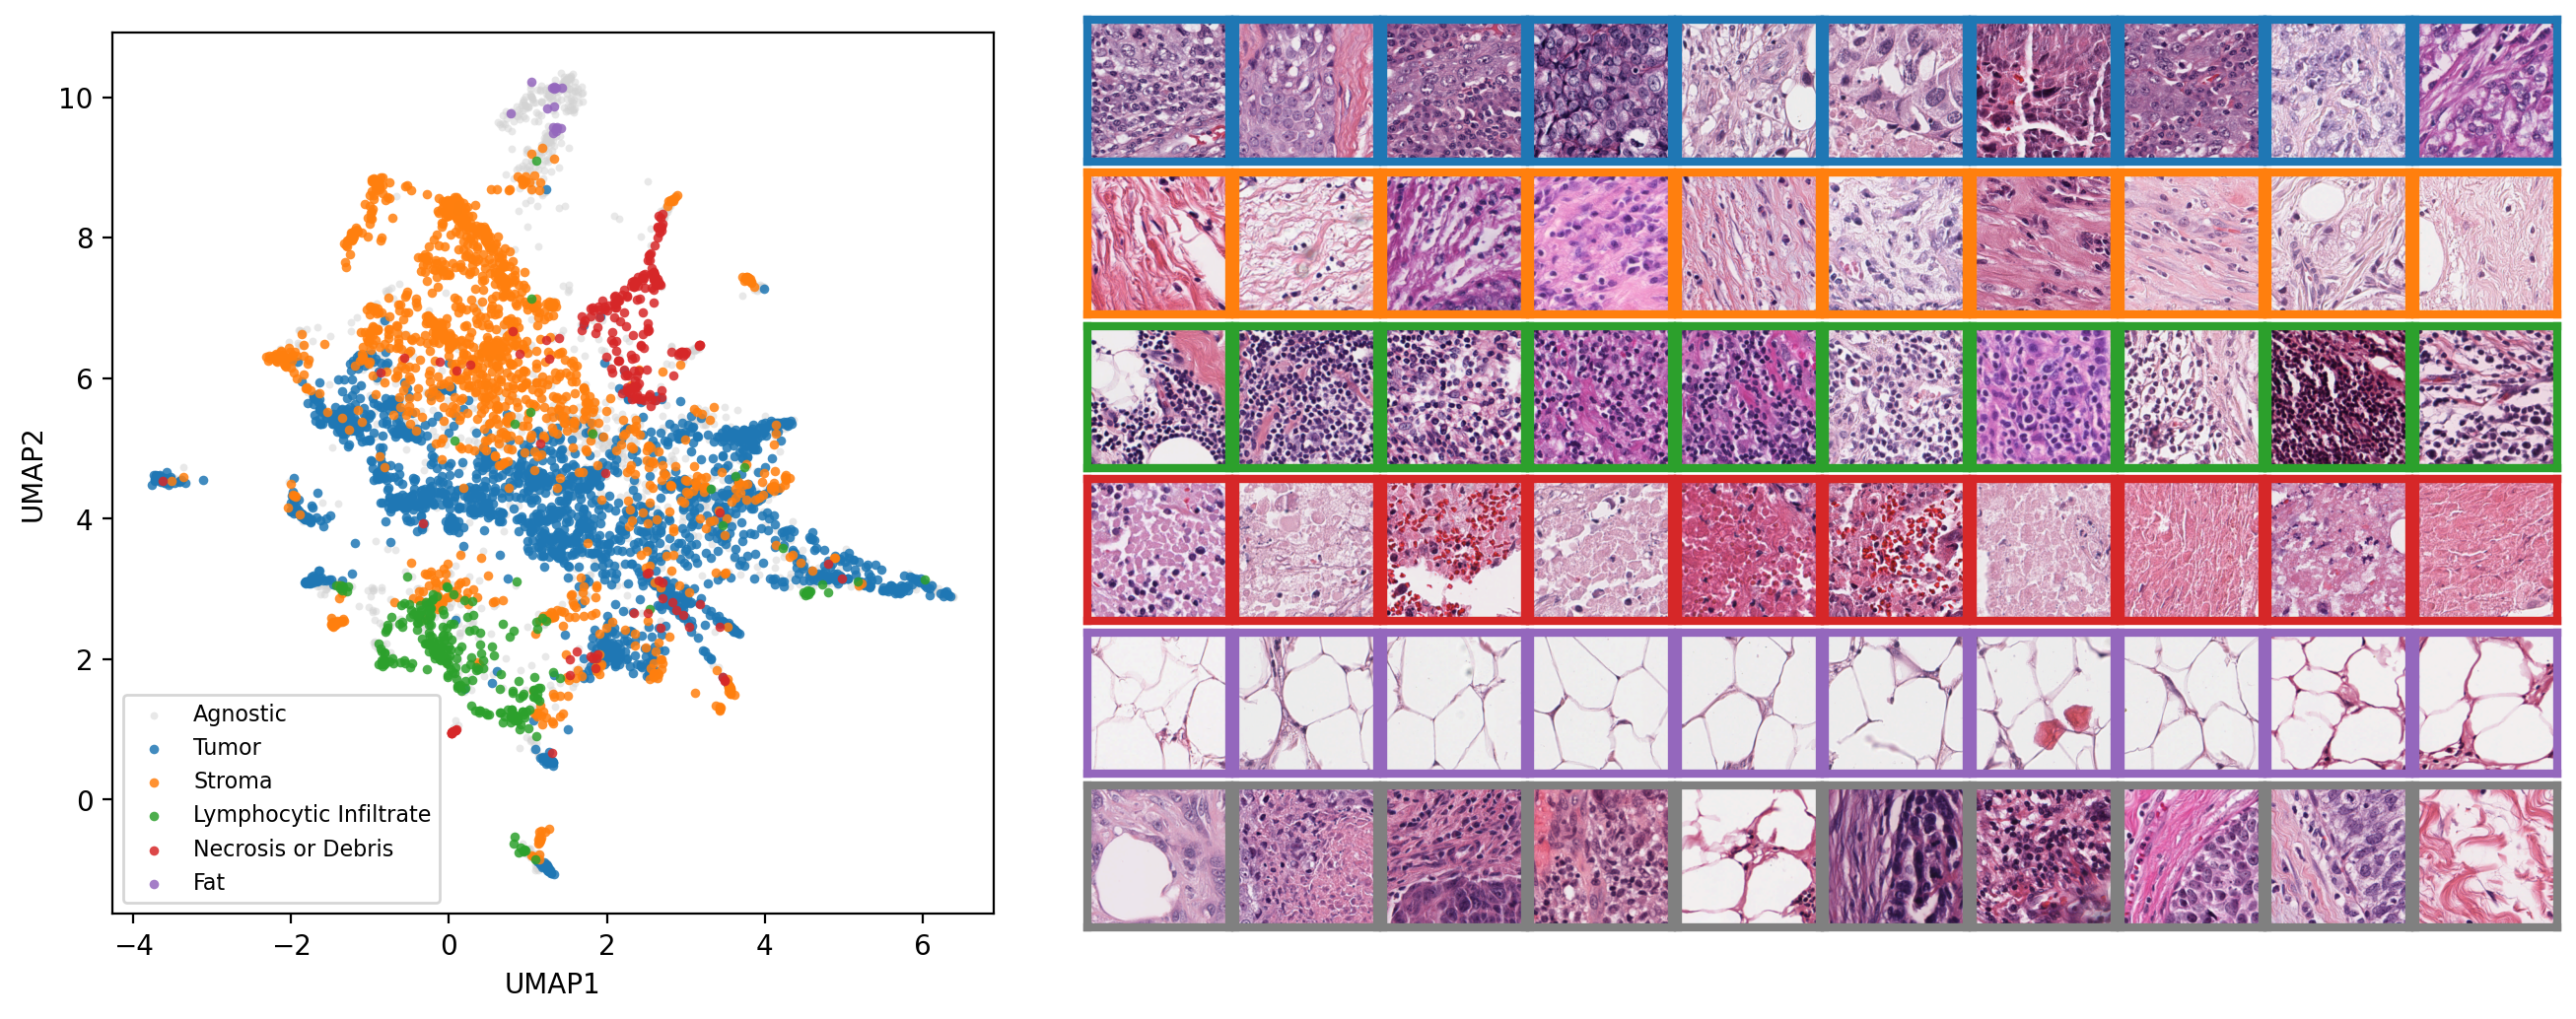
\includegraphics[width=1.0\linewidth]{images/resnet50-full_umap_encoder_model-prediction_top-5.png}
        \end{minipage}
    \end{subfigure}
    \begin{subfigure}{\textwidth}
        \centering
        \begin{minipage}[c]{0.05\textwidth}
            \rotatebox{90}{\textbf{Hematoxylin}}
        \end{minipage}
        \begin{minipage}[c]{0.7\textwidth}
            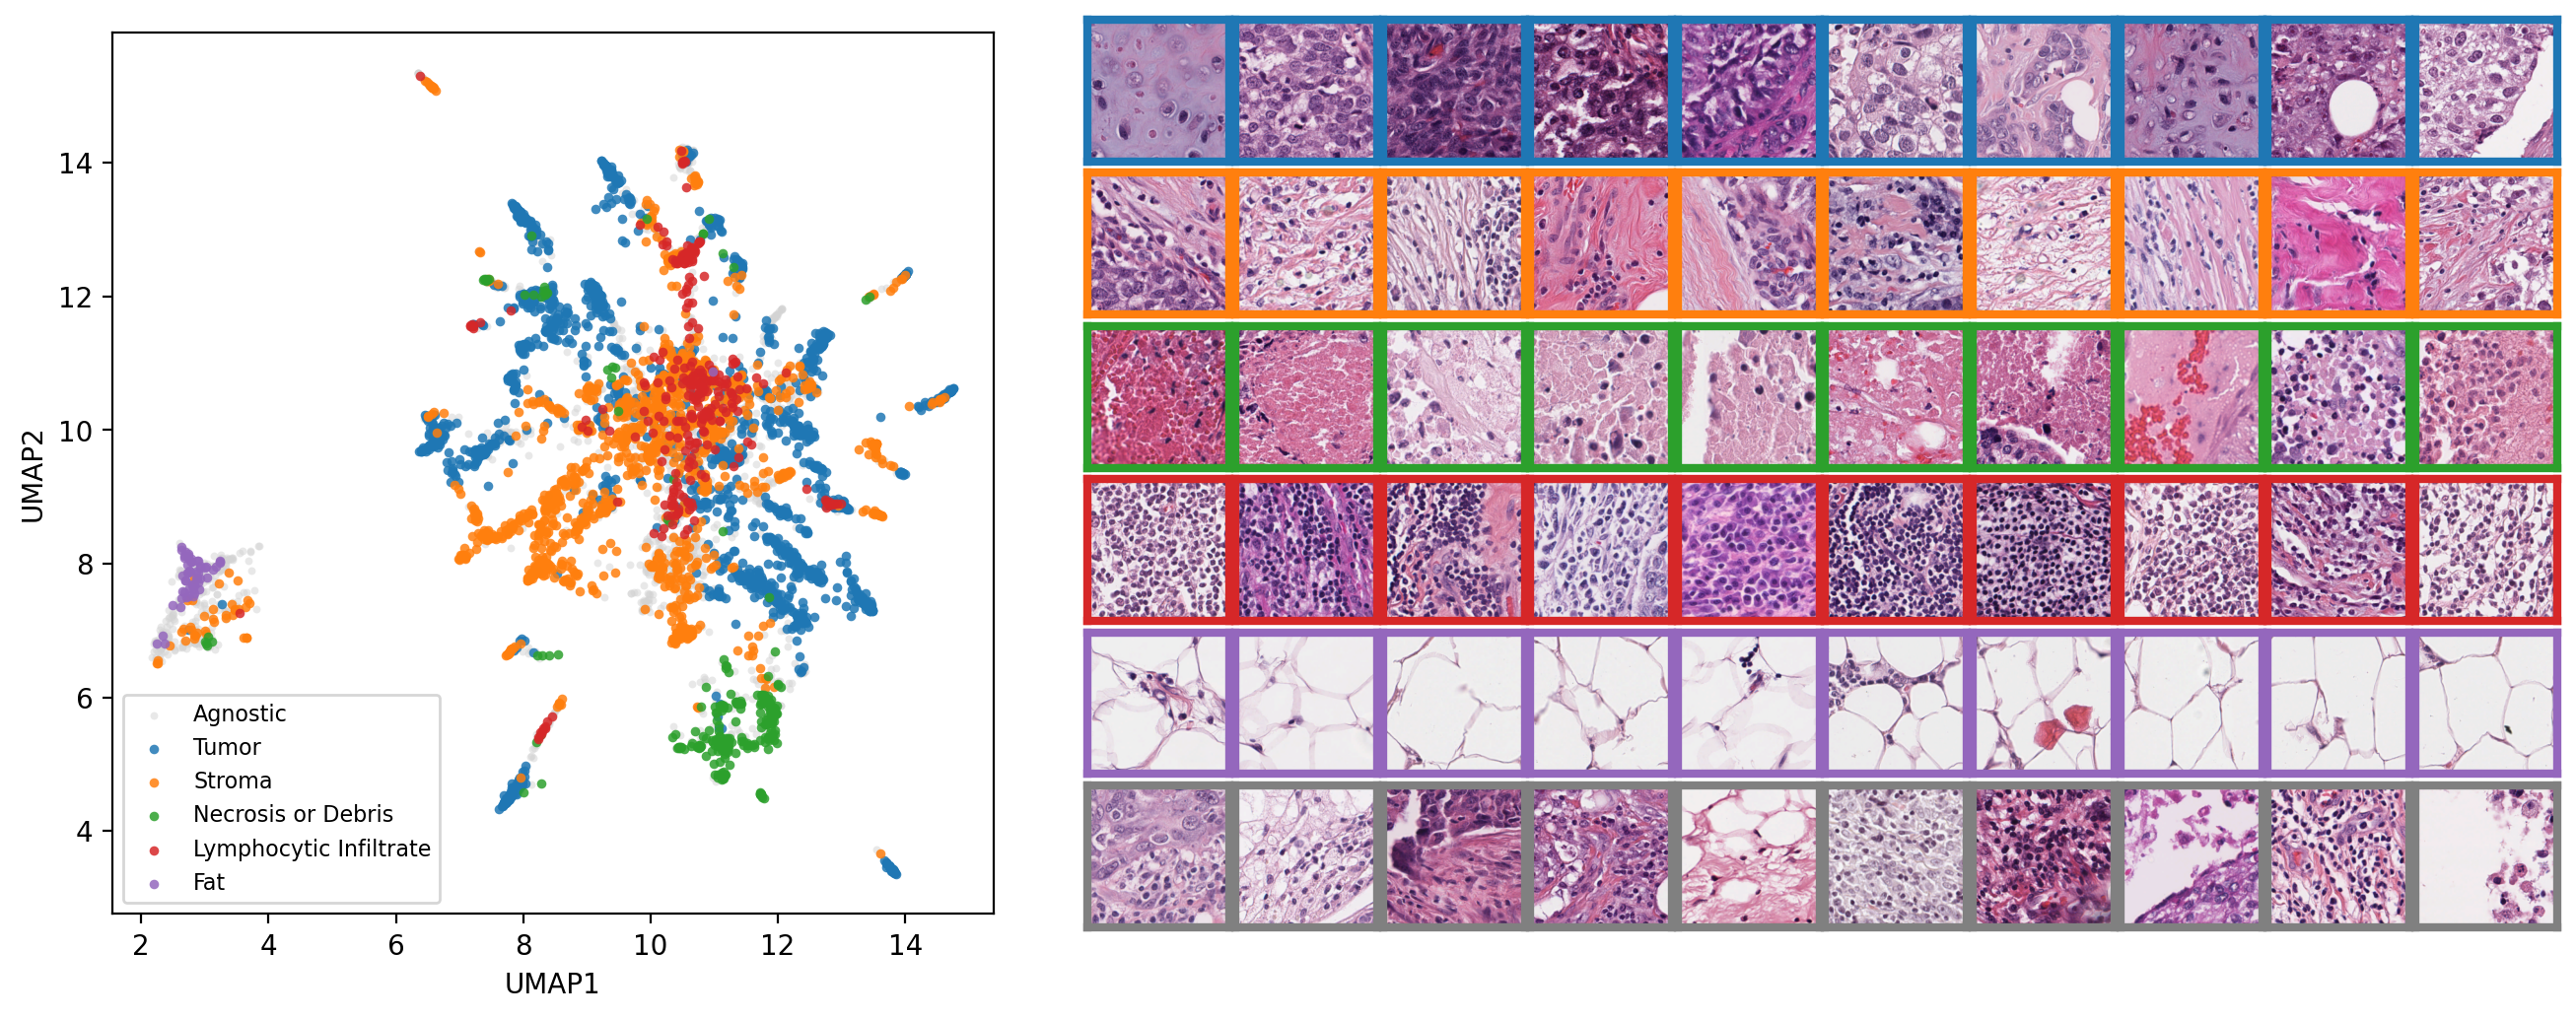
\includegraphics[width=1.0\linewidth]{images/resnet50-hematoxylin_umap_encoder_model-prediction_top-5.png}
        \end{minipage}    
    \end{subfigure}
    \begin{subfigure}{\textwidth}
        \centering
        \begin{minipage}[c]{0.05\textwidth}
            \rotatebox{90}{\textbf{JigMag}}
        \end{minipage}
        \begin{minipage}[c]{0.7\textwidth}
            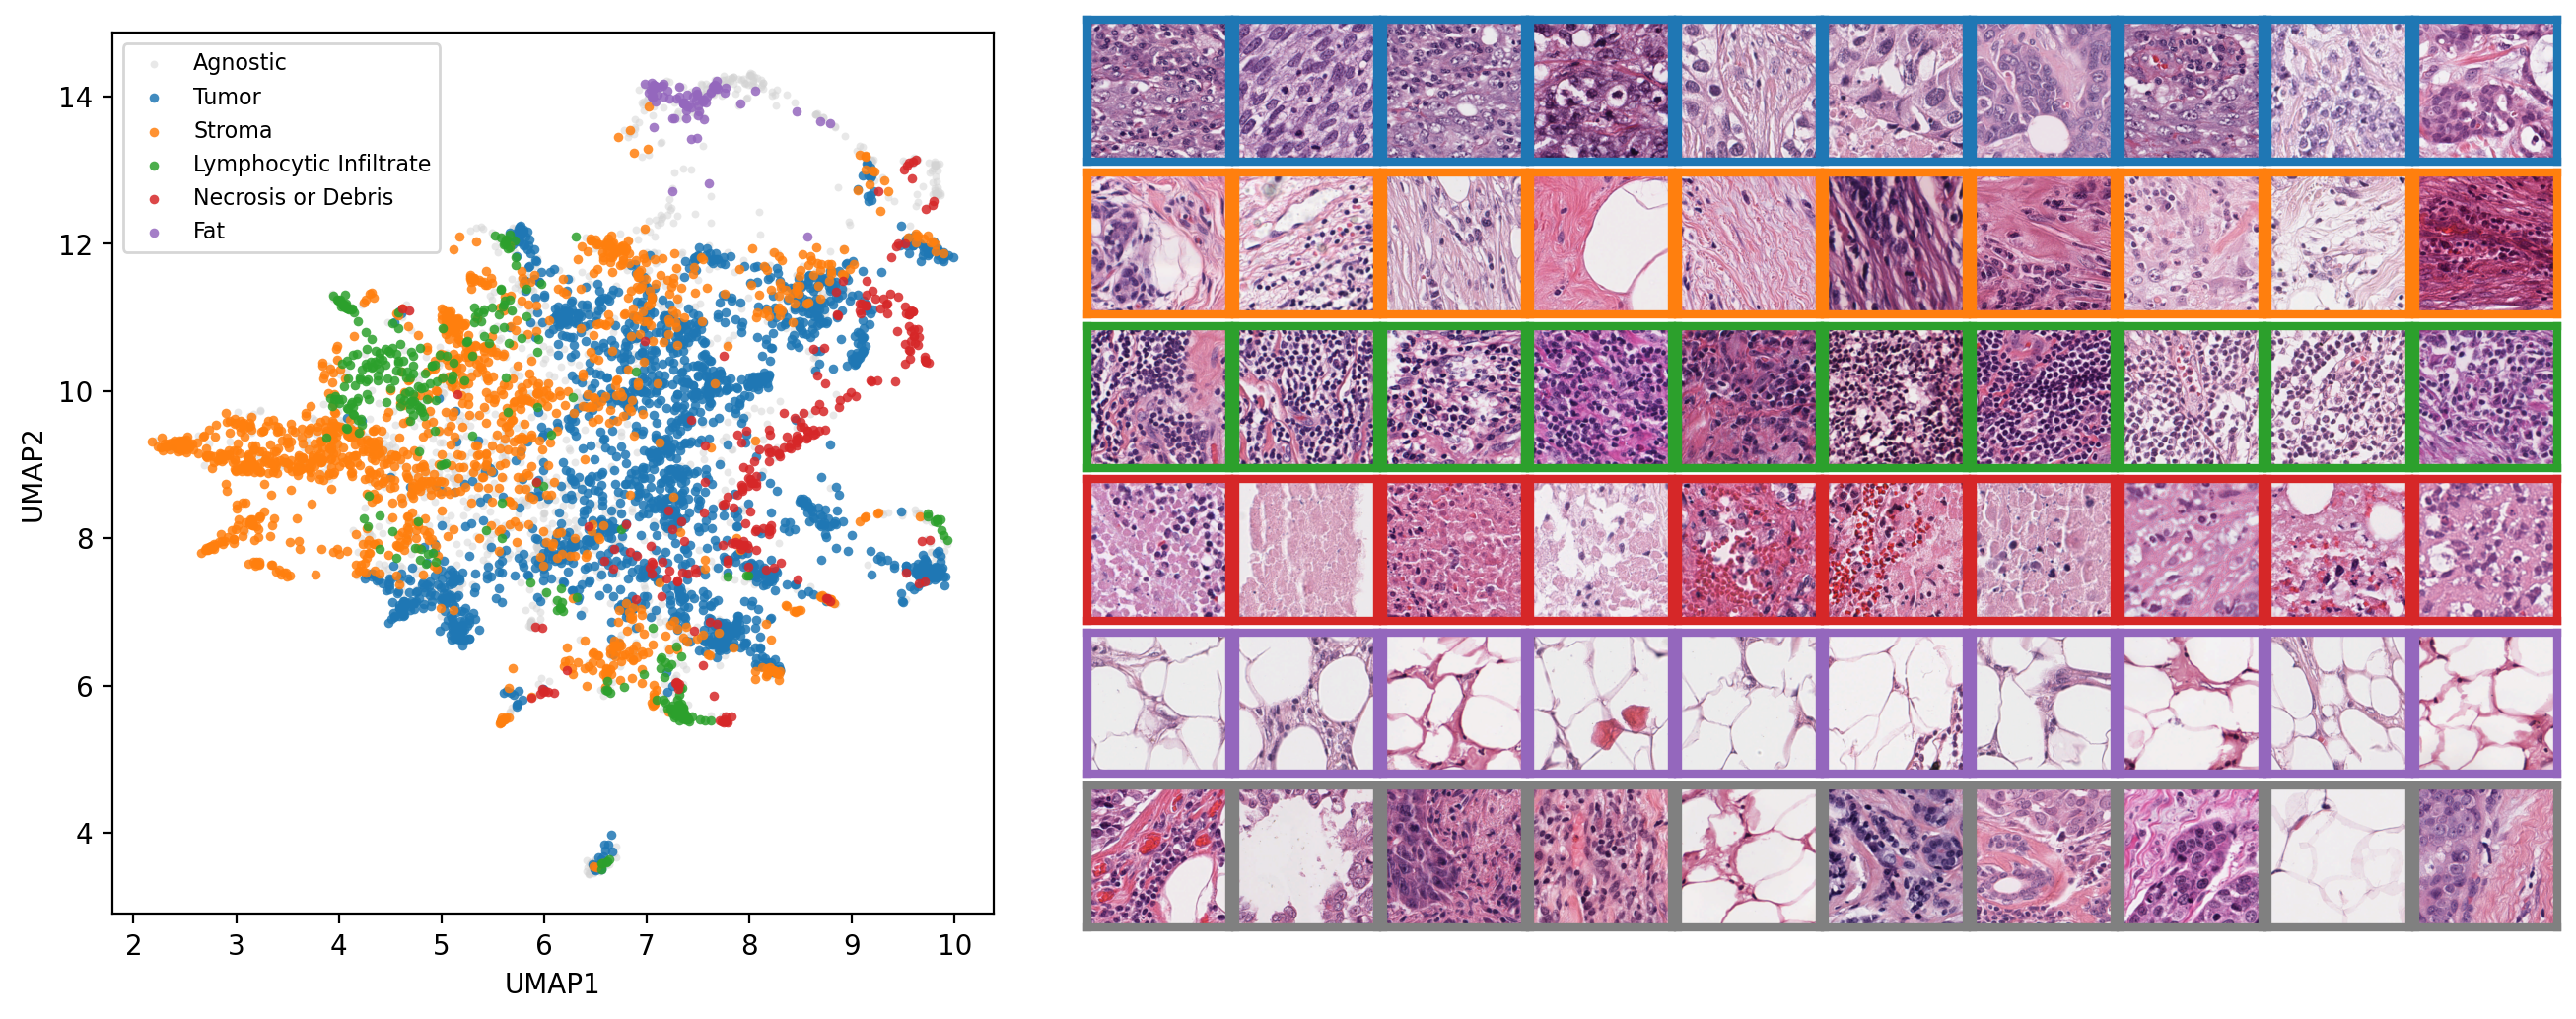
\includegraphics[width=1.0\linewidth]{images/resnet50-jigmag_umap_encoder_model-prediction_top-5.png}
        \end{minipage}    
    \end{subfigure}
    \begin{subfigure}{\textwidth}
        \centering
        \begin{minipage}[c]{0.05\textwidth}
            \rotatebox{90}{\textbf{Magnification}}
        \end{minipage}
        \begin{minipage}[c]{0.7\textwidth}
            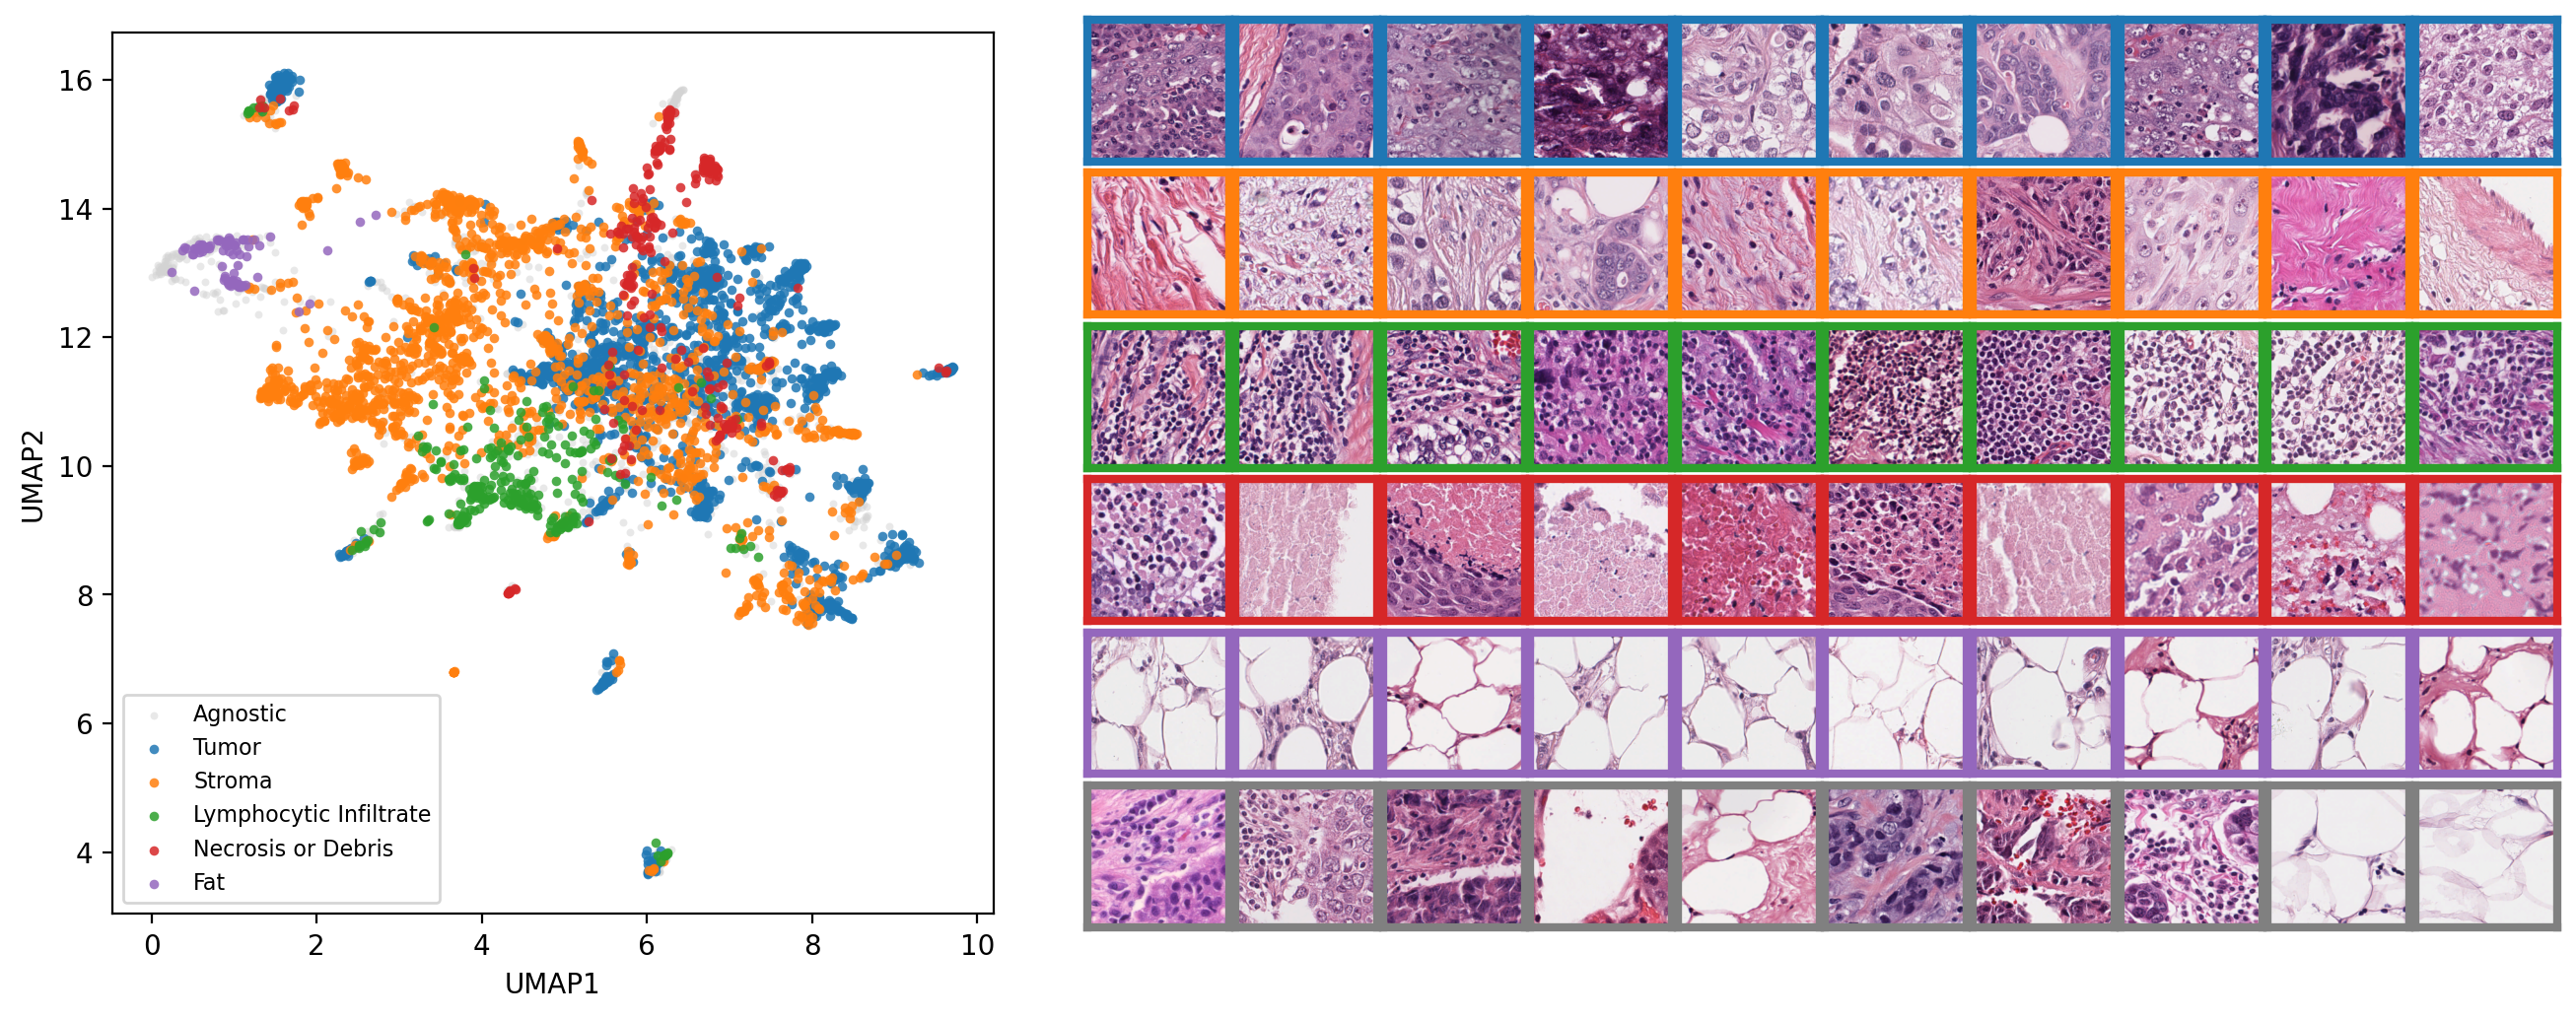
\includegraphics[width=1.0\linewidth]{images/resnet50-magnification_umap_encoder_model-prediction_top-5.png}
        \end{minipage}    
    \end{subfigure}
    \caption{\textbf{Visualization of the tile-level feature space after Stage 2.} For each pretext-task configuration, we randomly sampled 2\% of tiles from each slide in the independent test cohort and projected their 512-dimensional feature representations to two dimensions using UMAP. Each tile is shaded by its dominant tissue class, defined as the class whose proportion within the tile, as predicted by the tissue-segmentation tile encoder, is at least $p = 0.5$; tiles in which no class meets this threshold are labeled as ``Agnostic''. For clarity, we display only the five tissue classes that appear most frequently among the sampled tiles.}\label{fig:tile-featture-sapce}
\end{figure*}

\begin{figure*}
    \centering
    \begin{subfigure}{0.45\textwidth}
      
\includegraphics[width=\linewidth]{images/train_tile_learning_curves.png}
    \end{subfigure}
    \begin{subfigure}{0.45\textwidth}
        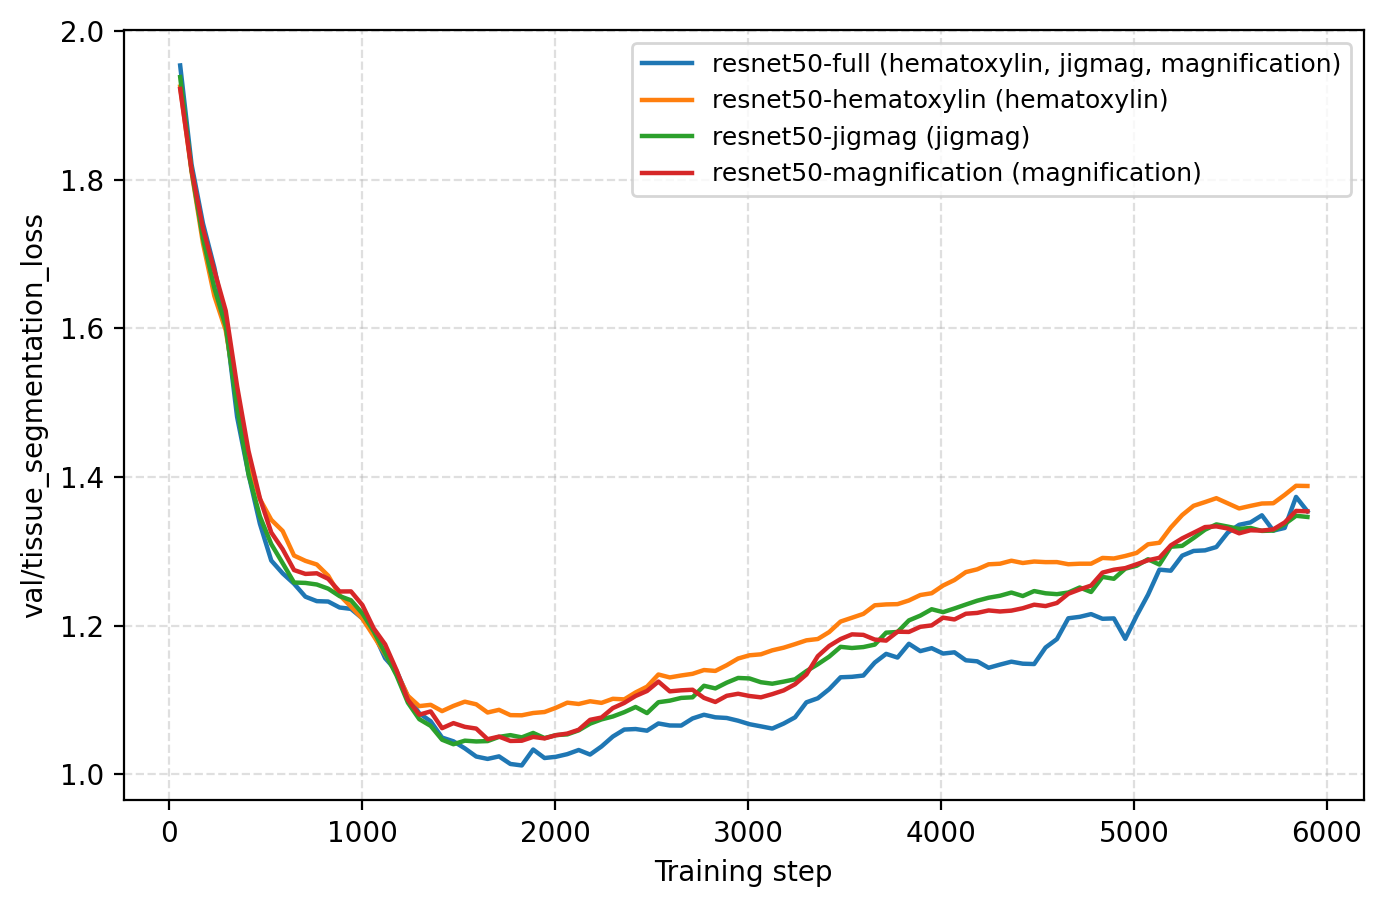
\includegraphics[width=\linewidth]{images/val_tile_learning_curves.png}
    \end{subfigure}
    \caption{\textbf{Tile-level tissue-segmentation learning curves across pretext-task configurations.} Training (left) and validation (right) tissue-segmentation loss over the course of Stage 2 training for the four pretext-task configurations: all pretext tasks combined, hematoxylin-channel prediction, JigMag, and magnification prediction. Each curve corresponds to one configuration; lower values indicate better tissue-segmentation performance.}
    \label{fig:tile-learning-curves}
\end{figure*}

\input{sections/discussion}
\input{sections/conclusion}


\bibliography{references}

\appendix



\end{document}
